\documentclass[crop,tikz]{standalone}
\usepackage[subpreambles=true]{standalone}

\usepackage{pgf, tikz}
\usetikzlibrary{arrows.meta,calc,decorations.markings,math,arrows.meta,patterns}

\pgfdeclarelayer{bg}
\pgfdeclarelayer{mg}
\pgfsetlayers{bg,mg,main}

\begin{document}

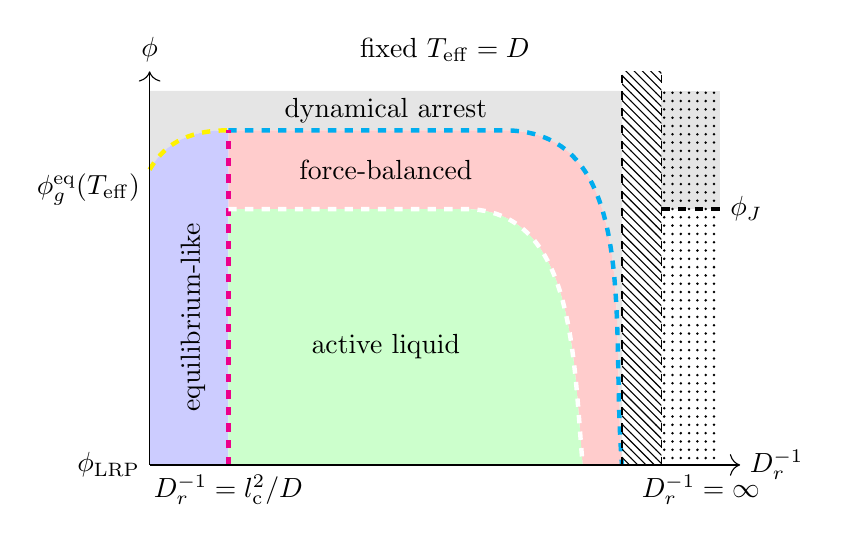
\begin{tikzpicture}[scale=0.5]

% axes
\draw[-{>[scale=1.5]}] (0, 0) -- (15, 0);
\draw (15, 0) node[right]{$D_r^{-1}$};
\draw[-{>[scale=1.5]}] (0, 0) -- (0, 10);
\draw (0, 10) node[above]{$\phi$};
\draw (0, 0) node[left]{$\phi_{\rm LRP}$};

% title
\draw (7.5, 10) node[above]{fixed $T_{\rm eff} = D$};

% separation to \infty
\draw[dashed] (12, 0) -- (12, 10);
\draw[dashed] (13, 0) -- (13, 10);
\fill[pattern=north west lines] (12, 0) rectangle (13, 10);
\draw (14, 0) node[below]{$D_r^{-1} = \infty$};

% jamming
\fill[pattern=dots] (13, 0) rectangle (14.5, 9.5);
\begin{pgfonlayer}{bg}
\fill[color=gray!20] (13, 6.5) rectangle (14.5, 9.5);
\end{pgfonlayer}
\begin{pgfonlayer}{mg}
\draw[color=black, ultra thick, dashed] (13, 6.5) -- (14.5, 6.5);
\end{pgfonlayer}
\draw (14.5, 6.5) node[right]{$\phi_J$};

% dynamical arrest
\begin{pgfonlayer}{bg}
\fill[color=gray!20] (0, 7.5) to[out=60,in=180] (2, 8.5) to [out=0,in=180] (9, 8.5) to[out=0,in=95] (12, 0) -- (12, 9.5) -- (0, 9.5) -- cycle;
\end{pgfonlayer}
\draw (6, 9) node{dynamical arrest};
\draw (0, 7) node[left]{$\phi_g^{\rm eq}(T_{\rm eff})$};

% force-balanced
\begin{pgfonlayer}{bg}
\fill[color=red!20] (2, 6.5) to[out=0,in=180] (8, 6.5) to [out=0,in=95] (11, 0) -- (12, 0) to[out=95,in=0] (9, 8.5) to[out=180,in=0] (2, 8.5) -- cycle;
\end{pgfonlayer}
\begin{pgfonlayer}{mg}
\draw[color=cyan, ultra thick, dashed] (2, 8.5) to [out=0,in=180] (9, 8.5) to[out=0,in=95] (12, 0);
\end{pgfonlayer}
\draw (6, 7.5) node{force-balanced};

% equilibrium-like
\begin{pgfonlayer}{bg}
\fill[color=blue!20] (0, 7.5) to[out=60,in=180] (2, 8.5) -- (2, 0) -- (0, 0) -- cycle;
\end{pgfonlayer}
\begin{pgfonlayer}{mg}
\draw[color=yellow, ultra thick, dashed] (0, 7.5) to[out=60,in=180] (2, 8.5);
\draw[color=magenta, ultra thick, dashed] (2, 0) -- (2, 8.5);
\end{pgfonlayer}
\draw (1.1, 3.75) node[rotate=90]{equilibrium-like};
\draw (2, 0) node[below]{$D_r^{-1} = l_{\rm c}^2/D$};

% active liquid
\begin{pgfonlayer}{bg}
\fill[color=green!20] (2, 6.5) to[out=0,in=180] (8, 6.5) to [out=0,in=95] (11, 0) -- (2, 0) -- cycle;
\end{pgfonlayer}
\begin{pgfonlayer}{mg}
\draw[color=white, ultra thick, dashed] (2, 6.5) to[out=0,in=180] (8, 6.5) to [out=0,in=95] (11, 0);
\end{pgfonlayer}
\draw (6, 3) node{active liquid};

\end{tikzpicture}

\end{document}
